\documentclass[12pt,a4paper]{article}
\usepackage[a4paper,width=150mm,top=25mm,bottom=25mm,bindingoffset=6mm]{geometry}
\usepackage[utf8]{inputenc}
\usepackage[portuguese]{babel}
\usepackage[T1]{fontenc}
\usepackage{amsmath}
\usepackage{amsfonts}
\usepackage{amssymb}
\usepackage{blindtext}
\usepackage{indentfirst}

\usepackage{tikz}
\usetikzlibrary{arrows}
\usepackage{verbatim}

\usepackage{graphicx}
\graphicspath{{images/}}

\begin{document}
\begin{titlepage}
	\begin{center}
		\vspace*{1cm}

		\Huge
		\textbf{Relatório de Sinais e Sistemas}\\
		\Large
		\textbf{2017.2}

		\vspace{0.5cm}
		\Large
		Trabalho 01 - Caderno de Exercícios

		\vspace{1.5cm}

		
\includegraphics[scale=0.8]{pucrio}

		\vspace{1.5cm}

		\normalsize
		\textbf{Fernando Homem da Costa - 1211971}\\
		\textbf{Pedro Escalfoni - 1321234}

		\vfill

		\Large
		Departamento de Elétrica\\
		Pontifícia Universidade Católica do Rio de Janeiro\\
		ENG1400 - Sinais e Sistemas\\
		\today

	\end{center}
\end{titlepage}

%\newpage
\tableofcontents
\newpage

\section{Introdução}
\addcontentsline{toc}{section}{Introdução}



\section{Questão 1}
\addcontentsline{toc}{section}{Questão 1}
Essa questão aborda conceitos básicos sobre construção de sinais e suas representação em um domínio específico. Sobre os sinais dessa questão, podemos afirmar que eles são discretos, ou seja, possuem a sua variável independente "n" pertencente ao domínio do tempo discreto, onde "n" $\in$  $\mathbb{Z}$ . Além disso, propõe que os alunos possam conhecer as representações gráficas de sinais básicos, como, impulso unitário, degrau unitário, rampa unitária e a exponencial, considerando o intervalo exigido.

	\subsection{Letra (A)}
	\addcontentsline{toc}{section}{Letra (A)}
			\begin{figure}[!ht]
				\centering
				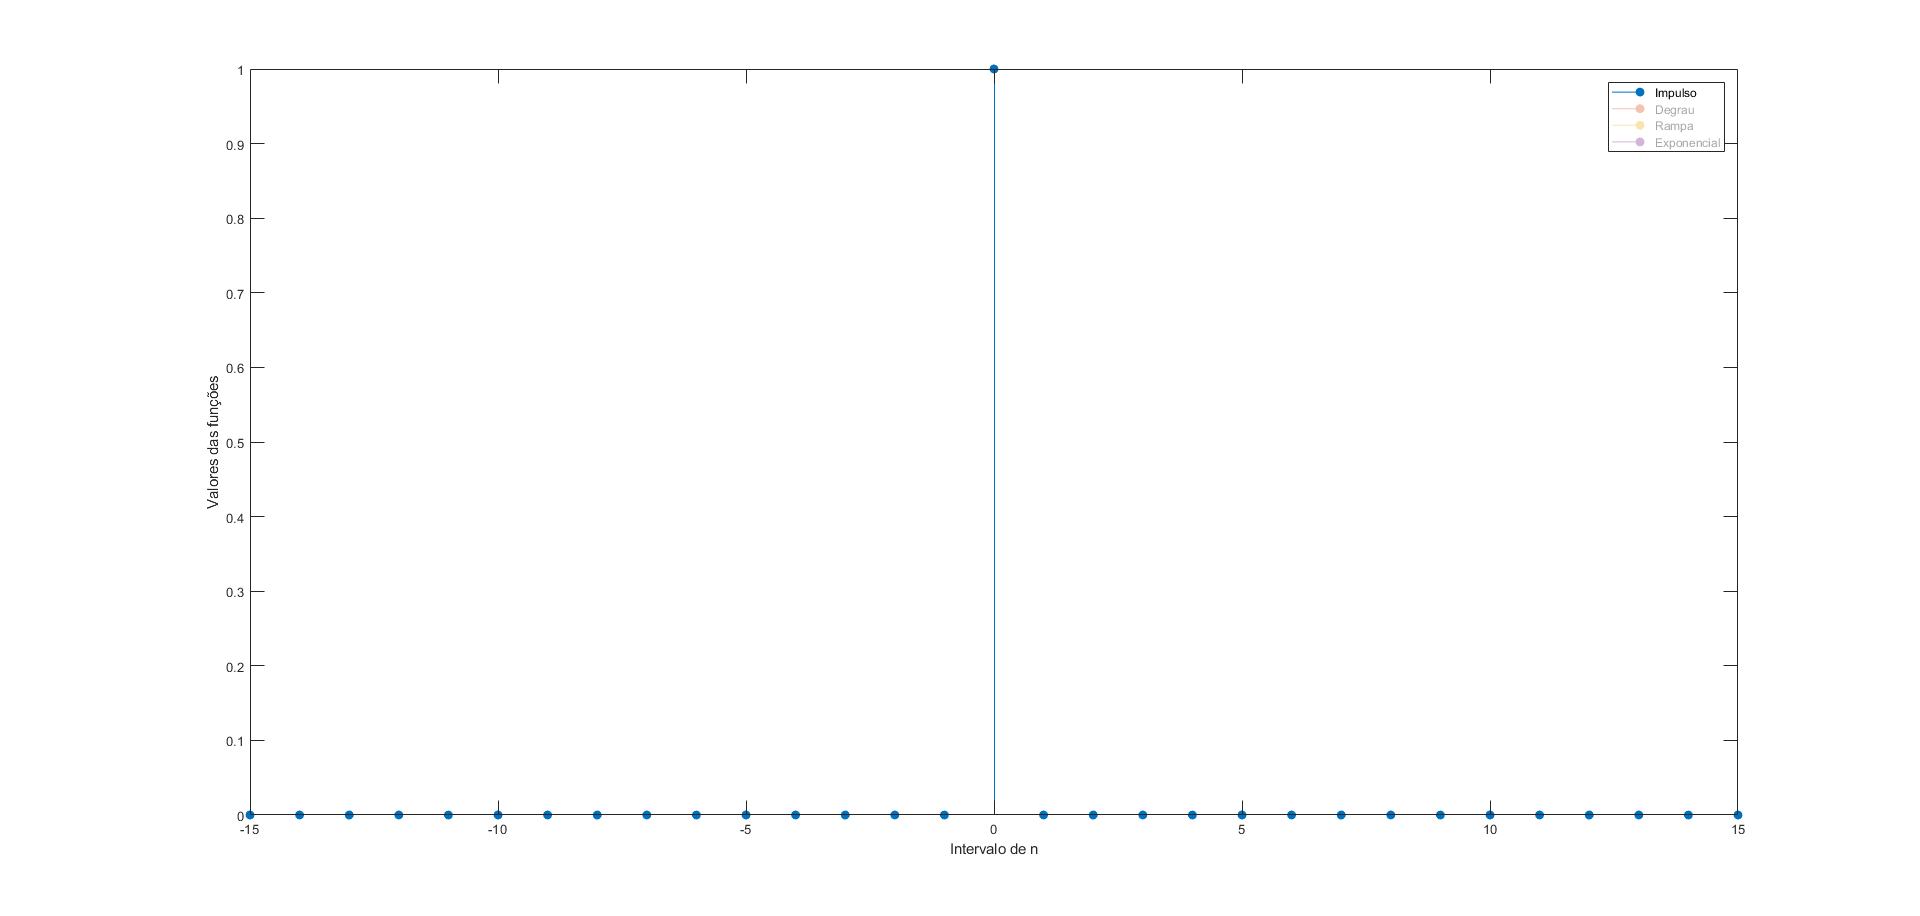
\includegraphics[width=\textwidth,scale=0.4]{1a-Imp}
				\caption{Gráfico - Impulso}
			\end{figure}
			\newpage

			\begin{figure}[!ht]
				\centering
				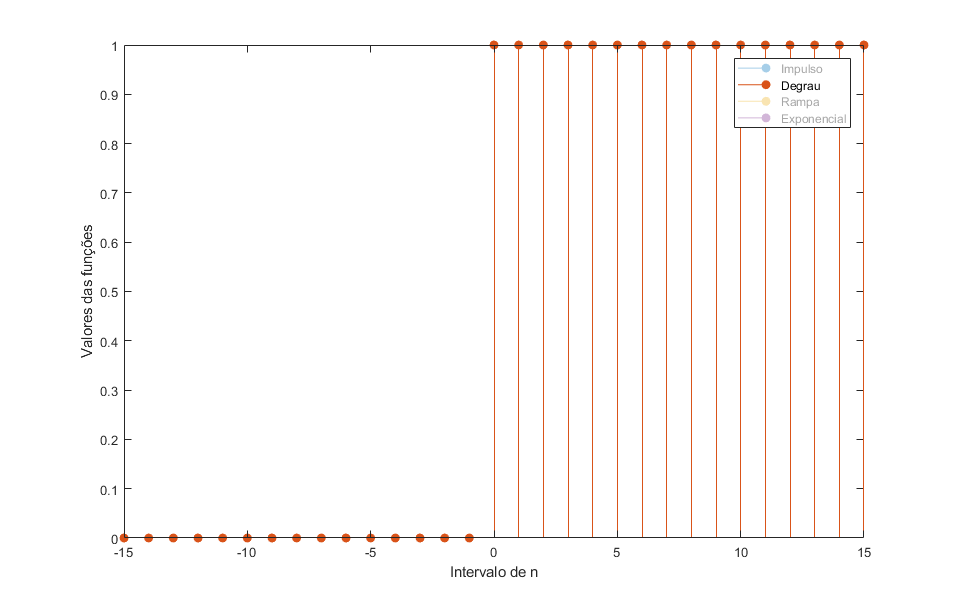
\includegraphics[scale=0.5]{1a-Deg}
				\caption{Gráfico - Degrau}
			\end{figure}

			\begin{figure}[!ht]
				\centering
				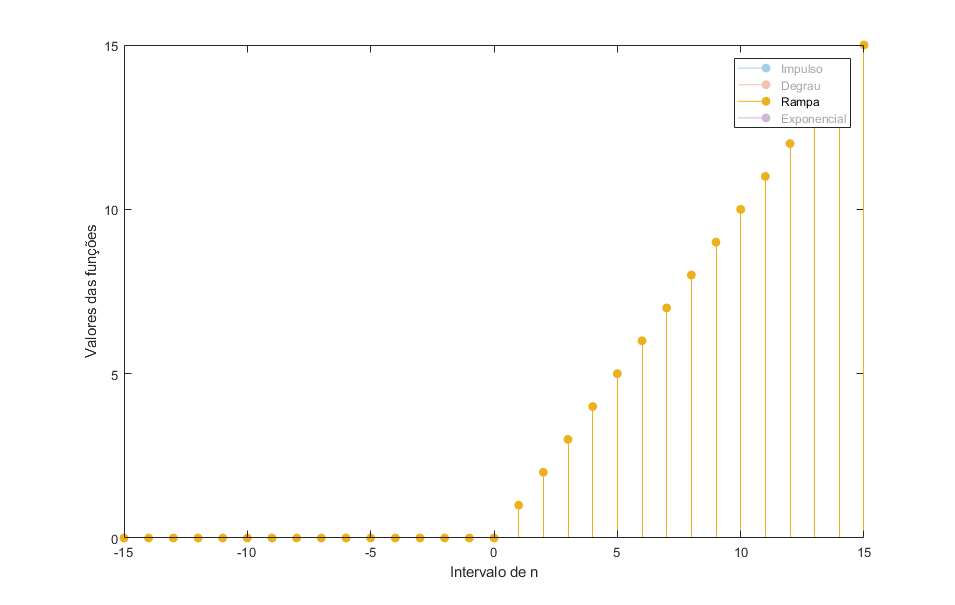
\includegraphics[scale=0.5]{1a-Ramp}
				\caption{Gráfico - Rampa}
			\end{figure}
			\newpage

			\begin{figure}[!ht]
				\centering
				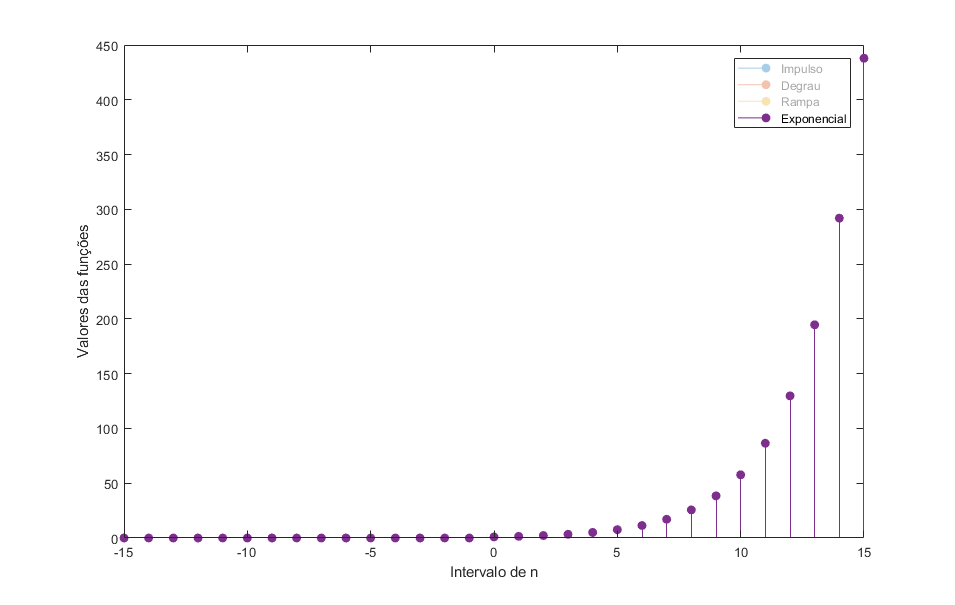
\includegraphics[scale=0.5]{1a-Exp}
				\caption{Gráfico - Exponencial}
			\end{figure}

			\begin{figure}[!ht]
				\centering
				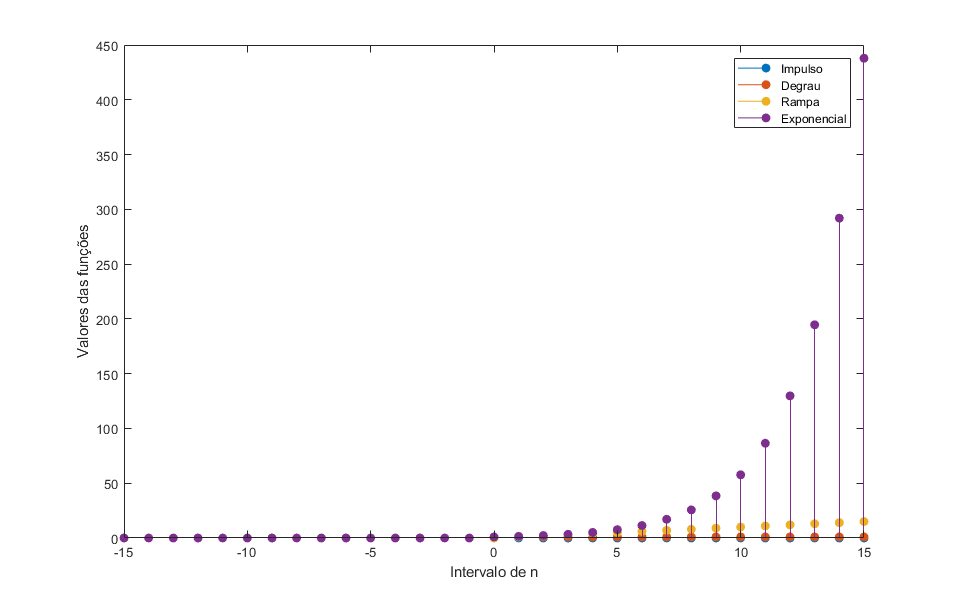
\includegraphics[scale=0.5]{1a-Tudo}
				\caption{Gráfico - Tudo}
			\end{figure}
			\newpage
	
	\subsection{Letra (B)}
	\addcontentsline{toc}{section}{Letra (B)}
	
	\subsection{Letra (C)}
	\addcontentsline{toc}{section}{Letra (C)}
			\begin{figure}[!ht]
				\centering
				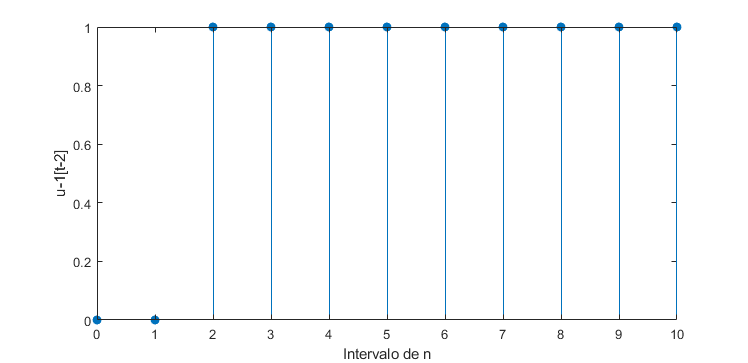
\includegraphics[scale=0.6]{1c-Deg1}
				\caption{Gráfico - Degrau}
			\end{figure}

			\begin{figure}[!ht]
				\centering
				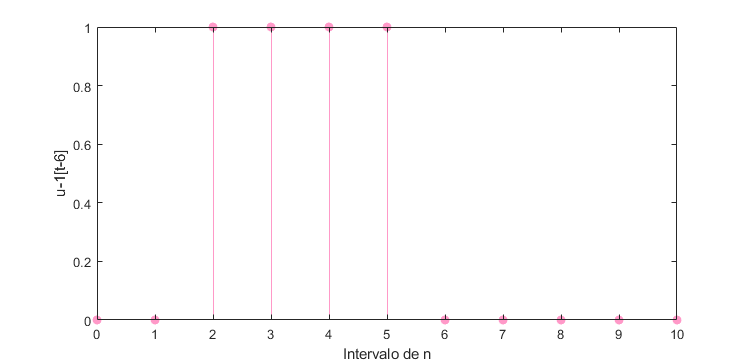
\includegraphics[scale=0.6]{1c-Deg2}
				\caption{Gráfico - Degrau}
			\end{figure}

			\begin{figure}[!ht]
				\centering
				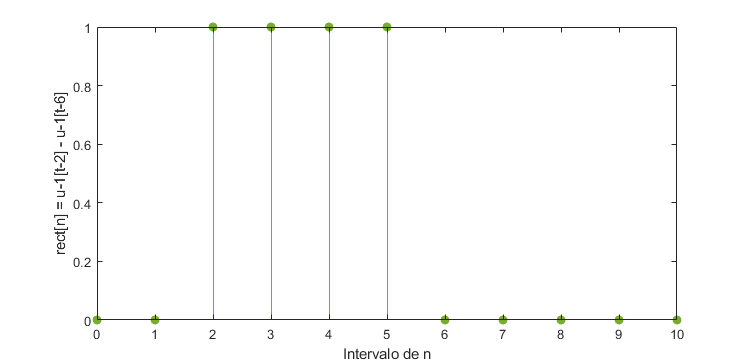
\includegraphics[scale=0.6]{1c-Rect}
				\caption{Gráfico - Rampa}
			\end{figure}
	
	\subsection{Letra (D)}
	\addcontentsline{toc}{section}{Letra (D)}


\section{Questão 2}
\addcontentsline{toc}{section}{Questão 2}
Essa questão aborda o conceito de periodicidade sobre funções. Dizemos que uma função é periódica, quando: f(k) = f(k + n*N), onde K $\in$, n $\in$ $\mathbb{Z}$, N $\in$ $\mathbb{Z}$ .
O objetivo é fazer com que o aluno coloque em prática esse conhecimento exigido por ela. Com isso, deve-se classificar as funções propostas pela questão em, periódicas ou aperiódicas, considerando o intervalo exigido.

\section{Questão 3}
\addcontentsline{toc}{section}{Questão 3}
Nessa questão podemos observar que muitos conceitos importantes estão sendo utilizados e relacionados entre si. O objetivo é obter o sinal de saída do sistemas através da convolução entre o sinal de entrada e a resposta impulsional. O primeiro fator importante abordado é de que se trata de um sistema linear invariante no tempo, ou seja, é um conjunto de operações matemáticas que não se alteram ao longo do tempo matemáticas e que só realizam operações lineares sobre os sinais de entradas afim de determinar o sinal de saída. O segundo fator é a resposta impulsional, que é saída de um sistema quando a entrada é um impulso. Por último, é a relação entre a entrada, a saída e a resposta impulsional do sistema, que por ser SLIT, podemos escrever a saída como a convolução entre o sinal de entrada e a resposta impulsional.
	\subsection{Letra (A)}
	\addcontentsline{toc}{section}{Letra (A)}
		\begin{figure}[!ht]
				\centering
				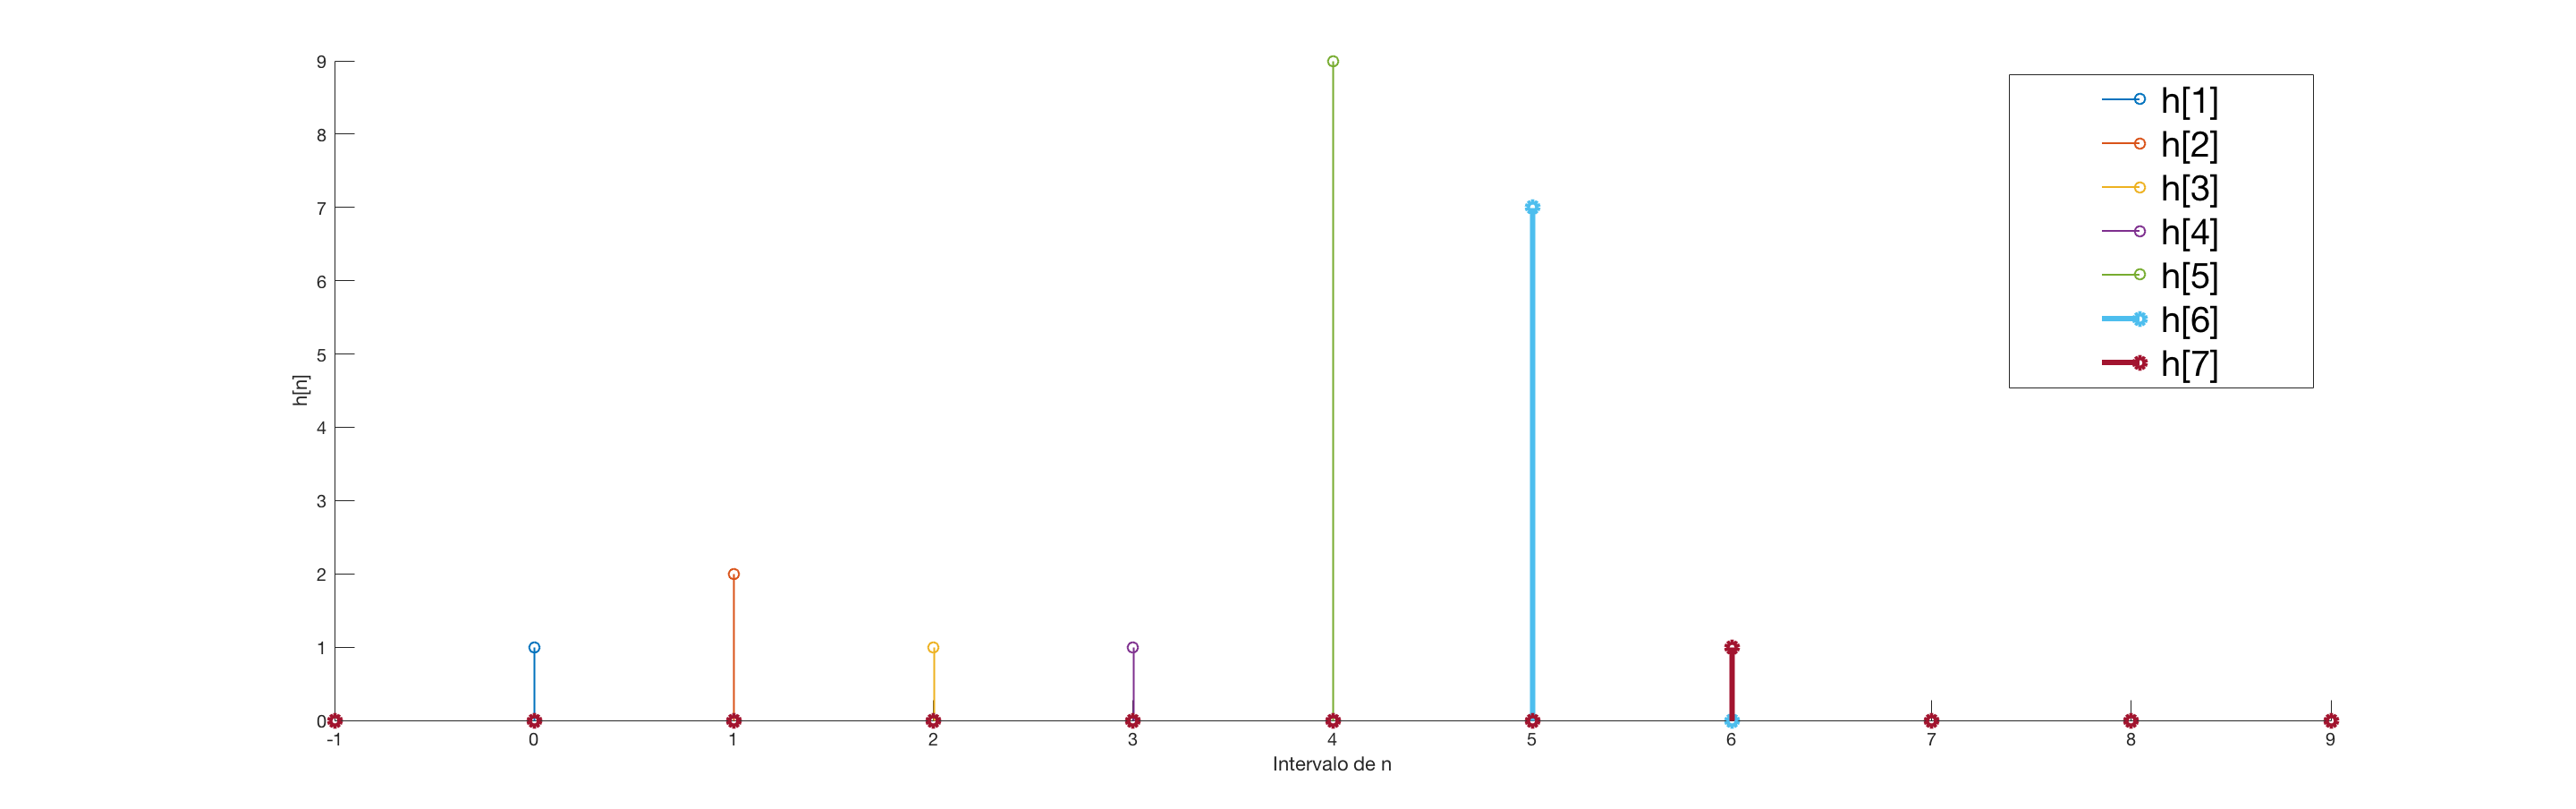
\includegraphics[width=\textwidth]{3a-respostaimpulsional}
				\caption{Gráfico - Resposta Impulsional}
		\end{figure}

\section{Questão 4}
\addcontentsline{toc}{section}{Questão 4}
Nessa questão utilizaremos os conceitos de transformada Z e equação de diferenças finitas. A transformada 
$\mathbb{Z}$ permite construir uma função a partir de uma série. Com isso, possibilitará transformar equações diferenciais finitas em equações algébricas.
Seja f(t) definida para t $\ge$ 0. A Transformada-Z da série \{f(nT)\} \text{é dada por:}
F(z) = $\mathcal{Z}\{f[n]\}$ = $\sum{_{n=0}^{\infty} f[n] z^{-n}}$

\section{Conclusão}
\addcontentsline{toc}{section}{Conclusão}

Quando necessário, os autores devem apresentar figuras, gráficos ou tabelas para apresentar os resultados obtidos e justificar suas conclusões. Todas as formas de apresentação não textual de resultados devem incluir uma legenda descrevendo em algumas palavras aquilo que está sendo representado. Essa descrição deve ser suficiente para que o leitor entenda qual a intenção dos autores na inclusão daquele item.

Gráficos, em especial, devem estar claramente anotados, incluindo indicação sobre o conteúdo dos eixos, título e legenda caso necessário. Atenção para que as figuras não se sobreponham ao texto.

Seguem alguns exemplos de gráficos e tabelas:

\section*{Índice Remissivo}
\addcontentsline{toc}{section}{Índice Remissivo}

\end{document}

